\documentclass[11pt, oneside]{article}   	% use "amsart" instead of "article" for AMSLaTeX format
\usepackage{geometry}                		% See geometry.pdf to learn the layout options. There are lots.
\geometry{letterpaper}                   		% ... or a4paper or a5paper or ... 
%\geometry{landscape}                		% Activate for for rotated page geometry
%\usepackage[parfill]{parskip}    		% Activate to begin paragraphs with an empty line rather than an indent
\usepackage{graphicx}				% Use pdf, png, jpg, or eps§ with pdflatex; use eps in DVI mode
								% TeX will automatically convert eps --> pdf in pdflatex		
\usepackage{amssymb}
\usepackage{amsmath}
\usepackage{parskip}
\usepackage{color}
\usepackage{hyperref}

\title{Convergence tests}
%\author{The Author}
%\section{}
%\subsection*{}
\date{}							% Activate to display a given date or no date

\graphicspath{{/Users/telliott_admin/Dropbox/Tex/png/}}
% \begin{center} 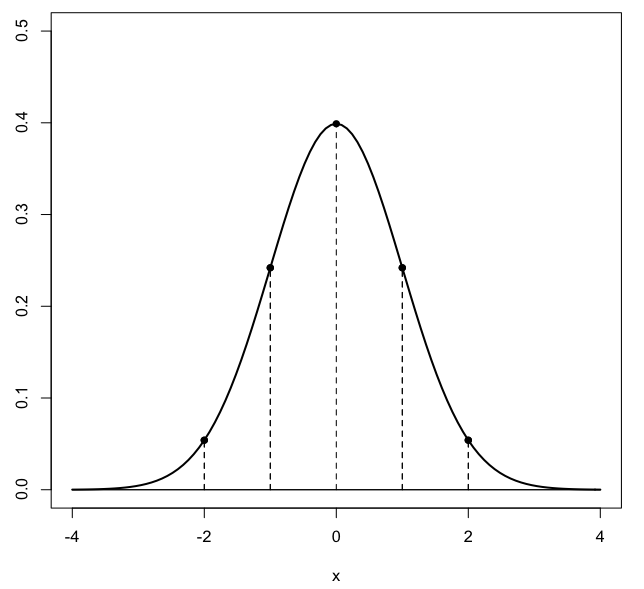
\includegraphics [scale=0.4] {gauss3.png} \end{center}
\begin{document}
\maketitle
\Large
\noindent
The most important series is the geometric series:
\[ s = \sum_{k=0}^{\infty} x^k \]
A famous example is $x=1/2$
\[ s = 1 + \frac{1}{2} + \frac{1}{4} + \frac{1}{8} + \dots \]

If we ignore the first term, and keep track of the sum after a number of terms, we see that at every step, the next step is to add precisely one-half of the difference between the current sum and the number $1$.  As a series, the cumulative sum is
\[ \frac{1}{2}, \ \frac{3}{4}, \ \frac{7}{8} , \ \frac{15}{16}, \ \dots \]
The limit is clearly equal to $1$.  Here is a visual proof
\begin{center}
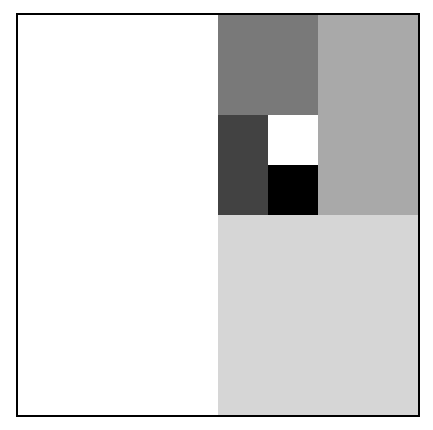
\includegraphics [scale=0.25] {series1.png}
\end{center}

If we assume that the series has a finite sum we can do the following:
\[ s = 1 + x + x^2 + x^3 + \dots \]
\[ sx = x + x^2 + x^3 + \dots \]
\[ s - sx = 1 \]
\[ s = \frac{1}{1-x} \]
In the case $x=1/2$, where we include the first term of $1$, we find that $s=2$ and this is consistent with what we had before.  

Another way to check this is to multiply out
\[ 1 = (1-x) (1 + x + x^2 + x^3 + \dots) \]
On the right-hand side, for each term in the second factor, we multiply by $1-x$.  Provided $x < 1$ the terms $x^n$ as $n$ gets larger become smaller and smaller, and finally negligible.

Or use distributivity with the first factor.  We have
\[ 1= (1 + x + x^2 + x^3 + \dots) - x(1 + x + x^2 + x^3 + \dots) \]
Each term in the first series (after the $1$), has a matching identical term with the factor of $-1$ in the series on the right, which will cancel.  However, this depends on $x^n$ getting smaller and smaller as $n \rightarrow \infty$, which only happens for $x < 1$.  In the limit, everything cancels except the $1$ in front.

The more formal way to do this is to compute the sum to $n$ places, for finite $n$:
\[ s_n = 1 + x + x^2 + x^3 + \dots + x^n \]
This sum is definitely finite.  Then we have
\[ s_n x = x + x^2 + x^3 + \dots + x^{n+1} \]
\[ s_n - s_n x = 1 - x^{n+1} \]
\[ s_n = \frac{1}{1-x} - \frac{x^{n+1}}{1-x} \]

Now, in the limit as $n \rightarrow \infty$, we see that the second term vanishes $\iff |x| < 1$.  For $x=1$ the sum is not defined.  For $x>1$ the sum goes to infinity.  We say it diverges.  For $x < -1$, the sum alternates sign, but each term gets larger in absolute value.  This case is also divergent.  We say that the geometric series has a radius of convergence $|x| < 1$.
\subsection*{series related to the geometric series}
\[ s = 1 + x + x^2 + x^3 + \dots \]
Differentiate
\[ 1 + 2x + 3x^2 + 4x^3 + \dots \]
\[ \frac{d}{dx} \ [ \ \frac{1}{1-x} \ ] \ = \frac{1}{(1-x)^2} \]
Check by multiplying out
\[ (1-x) (1 + 2x + 3x^2 + 4x^3 + \dots ) \]
\[ = 1 + 2x - x + 3x^2 - 2x^2 + 4x^3 - 3x^3 +  \dots ) \]
\[ = 1 + x + x^2 + x^3 + \dots \]
And since
\[ (\frac{1}{1-x})(\frac{1}{1-x}) = \frac{1}{(1-x)^2} \]
\[ (1 + x + x^2 + \dots) (1 + x + x^2 + \dots) \]
\[ = 1 + 2x + 3x^2 + 4x^3 + 5x^4 + \dots \]

Integrate
\[ \frac{1}{1-x} = 1 + x + x^2 + x^3 + \dots \]
\[ -\ln |1-x| = x + \frac{x^2}{2} + \frac{x^3}{3} + \dots \]
Substitute $-x$ for $x$
\[ \frac{1}{1+x} = 1 - x + x^2 - x^3 + \dots \]
Integrate
\[ \ln |1+x| = x - \frac{x^2}{2} + \frac{x^3}{3} - \frac{x^4}{4} + \dots \]
\[ \ln 2 = 1 - \frac{1}{2} + \frac{1}{3} - \frac{1}{4} + \dots \]
This series converges pretty slowly.

\subsection*{Tests for convergence}
Series like the Taylor series can be very helpful in approximating a function.  Here we review some common tests to see whether the sum of an infinite series converges to a finite limit, or instead diverges.

Start with the geometric series
\[ \sum_{k=0}^{\infty} x^k \]
Suppose we compute the sum of a number of terms $n$
\[ s_n = x^0 + x^1 + x^2 + \dots + x^n \]
Since this is a finite series, the sum exists so
\[ x s_n = x^1 + x^2 + \dots + x^{n+1} \]
\[ (1-x) s_n = 1 + x^{n+1} \]
\[ s_n = \frac{1}{1-x} - \frac{x^{n+1}}{1-x}, \ \ \ x \ne 1 \]
Clearly, if $x>1$ then the second term is positive and $x^n \rightarrow \infty$ as $n$ gets large.  If $x<-1$ then the second term alternates in sign and its absolute value gets very large as $n$ gets large.  For $|n| < 1$, as $n \rightarrow \infty$, the second term vanishes and we have
\[ s_n = \frac{1}{1-x} \]
For example,
\[ \sum_{k=0}^{\infty} (\frac{1}{2})^k = \frac{1}{1-1/2} = 2 \]
\[ \sum_{k=0}^{\infty} (\frac{1}{3})^k = \frac{1}{1-1/3} = \frac{3}{2} \]
and so on.

A second famous series is the harmonic series
\[ \sum_{k=0}^{\infty} \frac{1}{k^p} \]
especially with $p=1$
\[ \sum_{k=0}^{\infty} \frac{1}{k} = 1 + \frac{1}{2} + \frac{1}{3} + \dots \]
This series diverges.  

One proof is the following.  Assume that the series converges.  Then its sum has sum limit which we can call $L$.
\[ L = 1 + \frac{1}{2} + \frac{1}{3} + \frac{1}{4} +  \frac{1}{5} +  \frac{1}{6} \dots \]
\[ > \frac{1}{2} + \frac{1}{2} + \frac{1}{4} + \frac{1}{4} +  \frac{1}{6} +  \frac{1}{46}  \dots \]
\[ = 1 + \frac{1}{2} + \frac{1}{3} \dots \]
\[ = L \]
a contradiction.  Therefore, the harmonic series diverges.

Now let's look at some tests of convergence.

\subsection*{Divergence test}
The first test requires that the limit of the individual terms $a_k$ must tend to zero
\[ \lim_{k \rightarrow \infty} a_k = 0 \]
if not, then the sum diverges.  For example,
\[ \frac{1}{2} + \frac{2}{3} + \frac{3}{4} + \frac{4}{5} + \dots \]
This clearly diverges, since
\[ \lim_{k \rightarrow \infty} a_k = 1 \]
Or
\[ \lim_{k \rightarrow \infty} \frac{k}{2k + 1}, \ \ \ k \in \{1,2,\dots\} \]
\[ = \lim_{k \rightarrow \infty} \frac{1}{2 + 1/k} = \frac{1}{2} \ne 0 \]
Another example is the harmonic series
\[ \lim_{k \rightarrow \infty} \frac{1}{k} = 0, \ \ \ k \in \{1,2,\dots\} \]
Despite passing this test, the harmonic series diverges.  Thus, a pass is necessary but not sufficient.

\subsection*{Integral test}
The integral test says that a (well-behaved) function $f(x)$
\[ \int_1^{\infty} f(x) \ dx \]
converges $\iff$
\[ \sum_{k=1}^{\infty} f(k) \]
also converges.  The function must be continuous and ..

Let's apply this test to the harmonic series
\[ \sum_{k=0}^{\infty} \frac{1}{k} \]
We have
\[ \int_1^{\infty} x \ dx = \ln |x| \ \bigg |_1^{\infty} \]
but the upper bound has the limit
\[ \lim_{k \rightarrow \infty} \ln |k| = \infty \]
In general, for
\[ \sum_{k=0}^{\infty} \frac{1}{k^p} \]
if $p>1$, the sum converges, but not otherwise:
\[ \int_1^{\infty} x \ dx = \frac{1}{1-p}x^{1-p} \ \bigg |_1^{\infty} \]
For $p>1$
\[ \lim_{x \rightarrow \infty} x^{1-p} = 0 \]
On the other hand
\[ \int_1^{\infty} \frac{1}{n^2} \ dn = - \frac{1}{n} \ \bigg |_1^{\infty} = 0 - - 1 = 1 \]
so the $\sum 1/n^2$ converges.

\subsection*{Comparison test}
If we compare a series and a convergent series and the test series is smaller term-by-term, then it also converges.  Similarly, if a series is larger than a divergent series when compared term-by-term, it also diverges.  Any finite number of terms from the beginning of a series may be disregarded before starting the comparison.

Since
\[ \sum_{k=0}^{\infty} \frac{1}{k^2} \] 
converges, so does
\[ \sum_{k=0}^{\infty} \frac{1}{k^2 + 10} \] 
And since
\[ \sum_{k=0}^{\infty} \frac{1}{k} \] 
diverges, so does
\[ \sum_{k=0}^{\infty} \frac{1}{\ln|k+1|} \] 
since for $k>2$
\[ \ln|k+1| < k \]
 so
\[ \frac{1}{\ln|k+1|} > \frac{1}{k} \]

\subsection*{Ratio test}
Consider
\[ \sum_{k=0}^{\infty} a_k, \ \ \ a_k > 0 \] 
\[ \lim_{k \rightarrow \infty} \frac{a_{k+1}}{a_k} = L \]

\begin{displaymath}
   f(x) = \left\{
     \begin{array}{lr}
       L < 1 & : \text{converges} \\
       L > 1 & : \text{diverges} \\
	   L = 1 & : \text{inconclusive}
     \end{array}
   \right.
\end{displaymath} 
As an example
\[ \sum_{k=0}^{\infty} \frac{1}{k!} \]
Check
\[ \lim_{k \rightarrow \infty} \frac{1/(k+1)!}{1/k!} = \frac{1}{k+1} < 0 \]
This one is also easily checked by the comparison test since
\[ k! > k^2, \ \ \ k > 3 \]
Since $1/k^2$ converges, so does $1/k!$.

Or
\[ 1 + \frac{1}{2} + \frac{1}{3} + \frac{1}{4} + \dots \]
\[ \lim_{k \rightarrow \infty} \frac{1/n+1}{1/n} = \frac{n}{n+1} = 1 \]
so the test is inconclusive.

\end{document}  